\chapter{BrowserAudit as it stands}


\section{Initial project (V1)}

Charlie Hothersall's thesis can be found in \cite{charlie} , Browseraudit was built largely as a modification of Mocha with Chai assertion library \
Mocha was meant to be a nodejs testing library, but had browser support, hence allowed to have a base framework to save time and get the actual tests written \

It was really thought of as a Unit Testing framework code running on the browser which was in a way a valid analogy to Unit tests that the browser developers would \
have written for the implementation of security policies for their browsers, but of course here done at the client level. While Mocha helped save some time for the task and
it's asynchronous options were appreciated to save time running the tests; It did however need to be heavily customized with a rebuilt frontend using a Reporter interface that \
triggers callbacks on testStart end and Suite start and End.\ 

The frontend was beautifully done, making use of twitter bootstrap, with suitable design that didn't get in the way of understanding the tests, and that offered expandable\
information about the tests from just the name and category and Pass/fail down to the exact code and the assertions that fail or errors matching different users capabilities.\

There were a fair amount of basic tests of which the most notable one that illustrates an important tool for running these tests which is the img src property:
you can see this in action in \ref{fig:sop} 

\begin{figure}
\centering
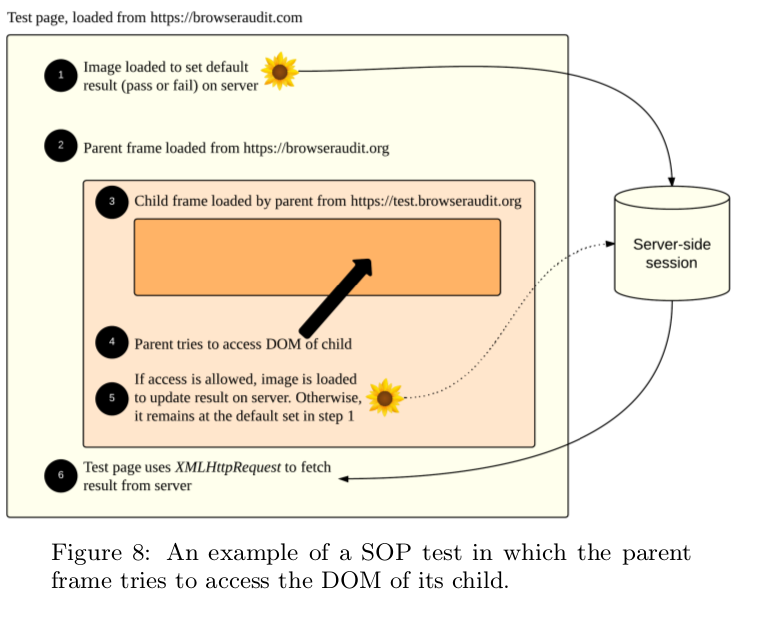
\includegraphics[width=1\textwidth]{./SOPbasic.png}
\caption{\label{fig:sop}Same origin policy typical test}
\end{figure}

As you can see the mechanism of img src property is used to communicate to the server on predefined appropriate pass/fail testiD endpoints. This is because 
the img object is not subject to any limitations and doesn't interfere in the testing of the security policy itself. This is used in many other types of tests.

The initial version had over 300 test tests and by using plain javascript and dilligently avoiding methods that are not adopted by most browsers,
The initial browseraudit version was supported and tested on these browsers:

\begin{itemize}
 \item Firefox desktop version 26, 29:  4 /306 and 6/306 failures respectively
 \item Android version 30: 14 failures
 \item Ie10: 74/306 failures issues running the actual tests, the failures are test implementation issues.
 \item Ie11: 64/306 In this instance some of the tests that failed in ie10 run but they are still failures.
 \item Safari Desktop version 6 and Ios Version: 6 /286 runs fast with few errors, less tests because no HSTS.
 \item Android 4.2.2: 64/267 problems with CORS and AJAX implementation
 \item Android 4.4.2: 2/286 failing test due to X-frame-Options ALLOW FROM not implemented.
\end{itemize}

Most notable discoveries of browseraudit were firefox's CSP implementation: CSP allows local CSS @import with only `unsafe-inline' set and 
CSP allows local Worker construction with only `unsafe-inline' set a very good spot that would have been very hard to detect in the wild!

\section{Current version adding tests (V2)}

Dr Sergio maffeis and Chris Novakovic took the project in hand and improved coverage drastically, there are now up to 404 tests and counting.
Matching the newer CSP standard, clickjacking and framebustig related tests etc..

The fact that Mocha was a nodejs package that had browser support started to show, because browser coverage is not terrific with the test framework.
Everybody had forgotten ie6 but ie8+ is considered a modern browser by many and we aim to be able to test any configuration in the wild, and ie at the time
of writing still represents 25+\% of the marketshare.\

For this reason the team decided to go for it's own test framework. which greatly simplifies the whole application, avoiding all the boiletplate that \
turned a unit testing framework into a browser based testing framework.

This current version , which we will refer to as (V2) is constantly being upgraded, and close integration with the code is required for my implementation\
but the new tiered architecture offers a simple modular way to deal with the tests which we will describe in the rest of this section. 

There is an intermediate version, V1.5, if you will, which was still running mocha and chai for test running but had all the extra tests written and \
was in the draft version of the browseraudit paper , available at \cite{maffeis}. We will only focus on the latest version because the framework and tests\
are thoroughly described in \cite{charlie}

\subsection{Test Backend in V2}

\subsubsection{Overall execution model}

Under the current version, categories, testsuites and tests are loaded from a postgres database, and test results "objects" are also saved on the database.
This is a Backend centric architecture which writes js hooks to the frontend.. the execution object models are loaded onto go code which generate javascript on the fly.
This javascript calls bridge functions similar to BrowserauditCategory(bla,bla,bla,bla) registering different categories and tests, it also passes their function invocation code \
with the correct html structures hardcoded as static assets.

This leaves to the frontend the sole mission to execute the code and update the UI with appropriate categories, descriptions, test suites, expected test  outcomes
and actual outcomes. Due to the way the tests are setup the outcome of those tests is known at the server endpoints as soon as the tests finish, leaving the 
go code that responds to the correct endpoint the task of also saving the feedback to the correct object in the database. 

It is also worthwhile to note that the go server sets up appropriate endpoints for the tests with the right testid etc from the database \
reflecting the different policies being tested, with a general pattern of different modules handling different types of requests and hence\
adding certain headers or responding a particular payload etc.\

\subsubsection{PostgreSQL model}

Take the time to check \ref{fig:model} the foreign keys have been conveniently marked with a diamond connector, we did not go into the details of suite execution settings.
because it was containing identical data in terms of displaymode this is a yet unused provision for future test suite display options among other settings.

As you can see there is a clear distinction to make between 
tests which belong to catgories and executions of browserAudit on users machines and the outcome of tests during those \
executions. This follows what was explained earlier about the execution model. As you can see everything about the tests is stored in database, which is the most sensible
approach for managing the sheer number of tests and providing maximum modularity concerning what we do with the data and how we add tests.\

It seems the way tests are currently being added is manually to the database and this is manageable since the data model is simple enough, but the first step we will
take is to improve on this and make our own interface to add tests in order to simplify all this, see \ref{label:addtest}.

\begin{figure}
\centering
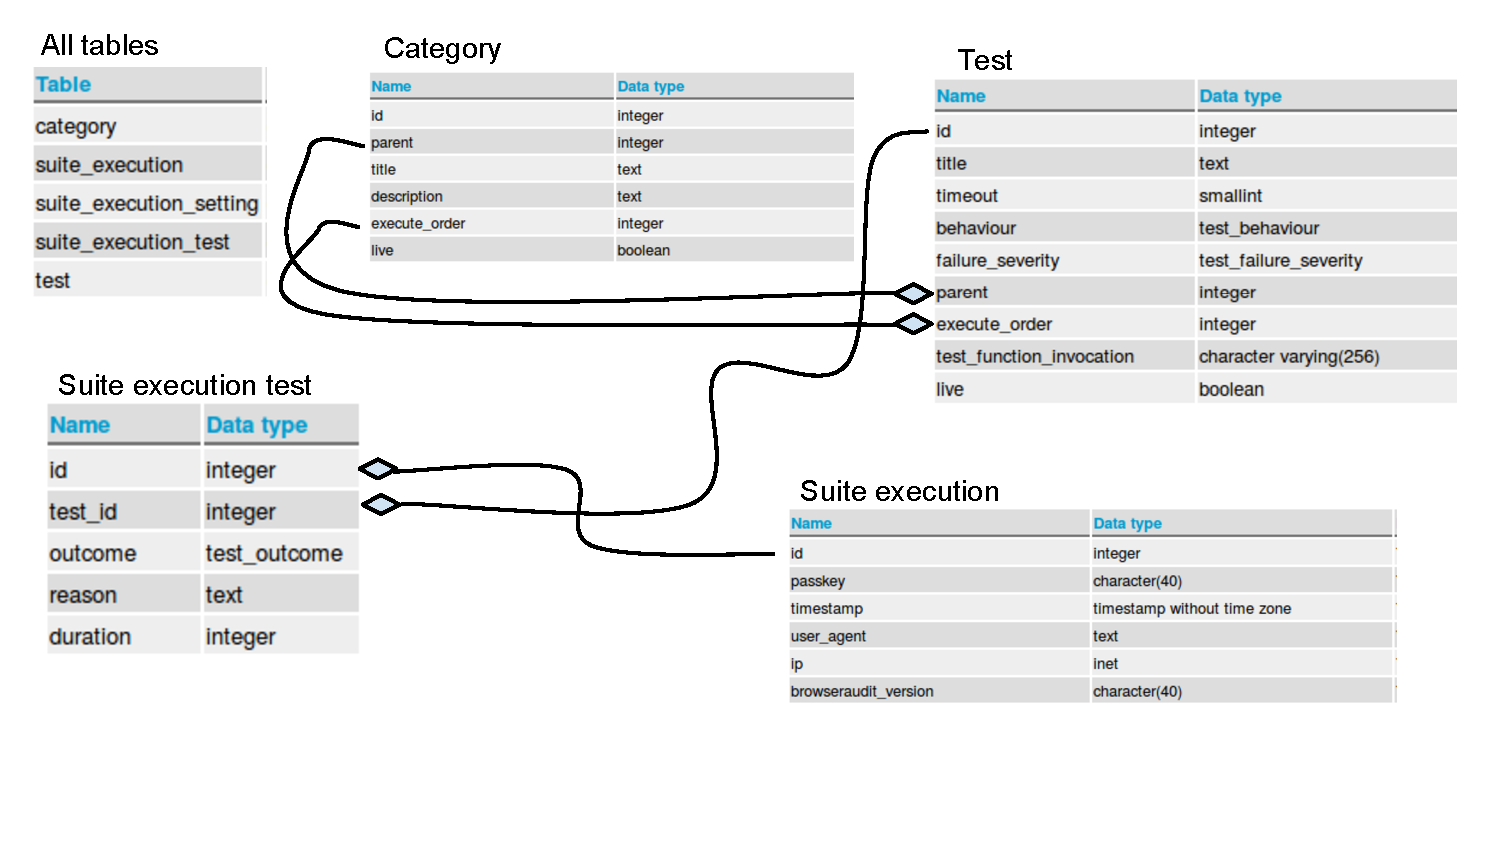
\includegraphics[width=1\textwidth]{db.pdf}
\caption{\label{fig:model}Database description of most important tables.}
\end{figure}


\subsubsection{The server}

\emph{Nginx}

There is an Nginx reverse proxy serving the static content and caching where cache directives are to allow caching for a response. this is thoroughly explained both in 
\cite{charlie} and \cite{maffeis}. an Apache 

\emph{the Go server}

As we discussed earlier the Go server handles the responses at the appropriate endpoints for the types or categories of tests. As we said in the model section, what is 
actually saved in the database in terms of test execution is the invocation of the right function types with suitable parameters and identification for later logging of results.
We will now go into the details of the client code that handles those classes of tests in section \ref{label:client}

\subsubsection{The Client test classes }
\label{label:client}

The client test classes are shown in the following table with the literal function names and short description \
these are the methods called by the tests that are in the database:

\begin{itemize}
 \item parentChildSopTest // Same-Origin Policy -> DOM access
 \item ajaxSopTest // Same-Origin Policy -> XMLHttpRequest
 \item domainScopeCookieTest // Same-Origin Policy -> Cookies - domain scope
 \item cookiePathScope // Same-Origin Policy -> Cookies - path scope
 \item cspTest //Content Security Policy
 \item originExpect // Cross-Origin Resource Sharing -> Access-Control-Allow-Origin  
 \item methodExpect // Cross-Origin Resource Sharing -> Access-Control-Allow-Methods
 \item headersExpect// Cross-Origin Resource Sharing -> Access-Control-Allow-Headers
 \item exposeExpect // Cross-Origin Resource Sharing -> Access-Control-Expose-Headers
 \item cookiesHttpOnlyServerToScript // Cookies -> HttpOnly flag -> HTTP-only cookie set by server and accessed from JavaScript
 \item cookiesHttpOnlyScriptToServer  // Cookies -> HttpOnly flag -> HTTP-only cookie set by JavaScript (should not be sent to server)
 \item cookiesSecureServerToScriptHTTPS // Cookies -> Secure flag -> cookie set by server should be sent over HTTPS
 \item cookiesSecureScriptToServerHTTP // Cookies -> Secure flag -> cookie set by JavaScript should not be sent over HTTP
 \item requestRefererHTTPSToHTTP // Request Headers -> Referer -> should not be sent over non-secure request if the referring page was transferred with a secure protocol
 \item frameOptionsTest // Response Headers -> X-Frame-Options
 \item hstsTest // Response Headers -> Strict-Transport-Security
\end{itemize}
